\documentclass[../main.tex]{subfiles}

\begin{document}

\subsection*{(1)}

取任意类$c$,
任意类$\tilde{c} (\forall \tilde{c} \ne c)$,
$x_c$ 为一$c$类样本

因为类$c$对其它类线性可分,
故$f(x_c, w_c^\star) > f(x_c, w_{\tilde{c}}^\star)$

显然, 对所有C个类, 都存在一个权重向量$w_c^\star, 1 \le c \le C$,
使得
$f(x_c, w_c^\star) > f(x_c, w_{\tilde{c}}^\star), \forall \tilde{c} \ne c$
成立

故训练集线性可分

\subsection*{(2)}

\begin{figure}
    \centering
    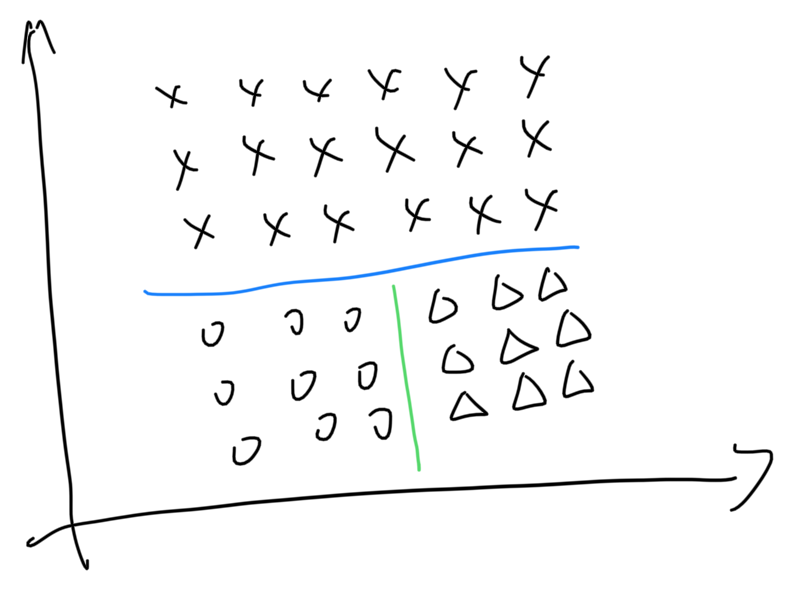
\includegraphics[width=.6\textwidth]{../figure/3-5.png}
    \caption{每两个类线性可分}
    \label{img3-5}
\end{figure}

如图\ref*{img3-5}所示,
叉, 三角, 圆为不同的三类, 其中两两线性可分,
但该数据集并不是线性可分的

\end{document}